\documentclass[dvipsnames, tikz]{standalone}
\usepackage{amsmath}
\usepackage{arevmath}
\usepackage{xcolor}
\usepackage{tikz}
\usetikzlibrary{calc}
\usetikzlibrary{decorations.pathreplacing,calligraphy,3d}
\usetikzlibrary{matrix,shapes,fit,backgrounds}

\begin{document}
	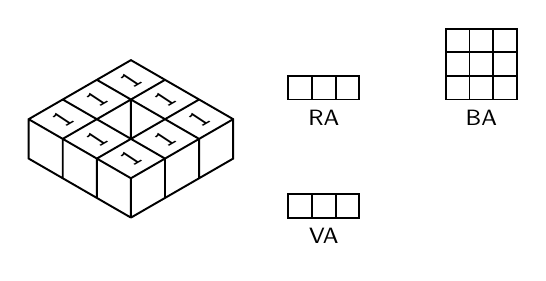
\begin{tikzpicture}[
		main/.style={
			line width=0.7pt,
			color=black
			}
		]
			
		\begin{scope}[scale=0.5, font=\small]
			\draw[main] (0,0) --++(30:3) --++(0,1) --++(150:3) --++(30:-3) --++(0,-1) --++(-30:3) (0,0) --++(0,1) --++(30:3) ++(30:-1) --++(150:3) ++(-30:1)++(30:1) --++(30:-3) ++(150:1) --++(-30:3) ++(30:1) --++(150:3) ++(0,-1) --++(0,-1) ++(-30:1) --++(0,1) --++(30:3) ++(0,-1) --++(0,-1) ++(30:-1) --++(0,1) ++(150:1) --++(0,1);
			\path (0,1.5) node[main, rotate=30,xslant=-0.5] {\sf 1};
			\path (30:1) ++ (0,1.5) node[main, rotate=30,xslant=-0.5] {\sf 1};
			\path (30:2) ++ (0,1.5) node[main, rotate=30,xslant=-0.5] {\sf 1};
			
			\path (30:1) ++ (0,2.5) node[main, rotate=30,xslant=-0.5] {\sf 1};
			
			\path (0,3.5) node[main, rotate=30,xslant=-0.5] {\sf 1};
			
			\path (-30:-1) ++ (0,1.5) node[main, rotate=30,xslant=-0.5] {\sf 1};
			\path (-30:-2) ++ (0,1.5) node[main, rotate=30,xslant=-0.5] {\sf 1};
			
			\path (-30:-1) ++ (0,2.5) node[main, rotate=30,xslant=-0.5] {\sf 1};
		\end{scope}
	
		\begin{scope}[xshift = 2cm, scale=0.3, font=\small]
			\draw[main] (0,0) --++ (3,0) --++(0,1) --++(-3,0) -- cycle (1,0) --++(0,1) ++(1,0) --++(0,-1);
			
			\path (1.5,0) node[main, below] {\sf \footnotesize VA};
		\end{scope}
		
		\begin{scope}[xshift = 2cm, yshift= 1.5cm, scale=0.3, font=\small]
			\draw[main] (0,0) --++ (3,0) --++(0,1) --++(-3,0) -- cycle (1,0) --++(0,1) ++(1,0) --++(0,-1);
			
			\path (1.5,0) node[main, below] {\sf \footnotesize RA};
		\end{scope}
		
		\begin{scope}[xshift = 4cm, yshift= 1.5cm, scale=0.3, font=\small]
			\draw[main] (0,0) --++(3,0) --++(0,3) --++(-3,0) -- cycle (1,0) --++(0,3) ++(1,0) --++(0,-3) (0,1) --++(3,0) ++(0,1) --++(-3,0);
			
			\path (1.5,0) node[main, below] {\sf \footnotesize BA};
		\end{scope}
	\end{tikzpicture}
\end{document}